\pdfinfo{
	/Author {Alex Lockwood}
	/Title {hw6}
	/Keywords {hw; hw6; 15-214}
}

\newcommand{\courseNum}{15-214}
%%%%%%%%%% FILL IN THE FOLLOWING INFORMATION %%%%%%%%%%
\newcommand{\hwNum}{6}
\newcommand{\hwTitle}{Building a Distributed Map/Reduce Framework}
\newcommand{\dueDate}{Thursday, May 1 at 11:59 p.m.}
%%%%%%%%%%%%%%%%%%%%%%%%%%%%%%%%%%%%%%%%%%%%%%%%%%%%%%%

\documentclass[11pt]{article}

\usepackage{geometry}
\usepackage[colorlinks=true]{hyperref}
\usepackage{fancyhdr}
\usepackage{graphicx}

\pagestyle{fancy}

\newenvironment{Section}[1]{
    \vspace{.25in}
    \noindent{\bf #1}
    \vspace{0.2em} \hrule \vspace {0.2in}
}

\newenvironment{SubSection}[1]{
    %\begin{samepage}
    \vspace{.1in}
    \noindent{\bf #1}
}{%\end{samepage}
}

\newcommand{\mtt}[1]{$\mathtt{#1}$}
\setlength{\parindent}{0in}
\setlength{\parskip}{0.1in}
\renewcommand{\headrulewidth}{0pt}

\lhead{\courseNum}
\rhead{Homework \hwNum}
\cfoot{\thepage}

\begin{document}

\begin{center}
{\Large Homework \#\hwNum: \hwTitle}\\
Due \dueDate
\end{center}

In this assignment you will implement a distributed map/reduce framework. 
Map/reduce is a programming model for processing large data sets, typically 
implemented by distributing a computation across multiple worker servers
where the data is stored. The computation is provided as a plug-in to the 
framework, and is specified as a separate map task and a reduce task. 
A client submits the two tasks to a master server, which is in charge of 
distributing the tasks across the worker servers in the system and 
returning the result back to the client when it is complete.

Your goals in this assignment are to:

\begin{itemize}
\item Gain a deep understanding of map/reduce and the challenges of
building a distributed system by implementing a map/reduce framework.
\item Learn how to use a map/reduce framework by implementing a simple
map/reduce task that uses your framework.
\item Practice network programming using {\tt Socket}s.
\item Practice parallel and concurrent programming in Java.
\end{itemize}

For this assignment we encourage you to discuss map/reduce and high-level
details of your solution with the course staff and with your 
classmates, but you may not share your code with other students
and must submit your own solution for the assignment.

\begin{Section}{Designing and implementing your map/reduce framework}

Your framework must match the basic architecture described
in lecture. Specifically, your framework should consist of three main components: 
a client, a master server, and multiple worker servers. The client simply submits the map and reduce tasks to the master server and waits for the master server to confirm that the computation is complete. 
Upon receiving the map and reduce tasks from the client, the master server manages the map/reduce computation, distributing the map and reduce tasks across a set of worker servers and specifying which worker servers should execute those tasks on which subsets of the data. The worker servers perform the actual work of the computation, each executing the map and reduce tasks on some subset of the data.

A map/reduce computation consists of two phases: a map phase and a reduce phase. In the map phase the master server distributes the map task across a set of worker servers.  The master server specifies on which subset of the data each map worker should execute the map task, and the map workers execute the map task on that subset of the data and write {\em intermediate results} to a file on their local disk.

After all map workers have completed the map task the master server
begins the reduce phase, distributing the reduce task across 
worker servers---sometimes but not necessarily the same set of workers that
executed the map task.  The master server specifies on which subset of the
intermediate results each reduce worker should execute the reduce task.
Each reduce worker begins by obtaining the specified subset of intermediate
results from the map workers, a step known as {\em the shuffle}.  In the
shuffle it's often necessary for every reduce worker to obtain some
intermediate results from every map worker; in practice implementing the 
shuffle efficiently is one of the most complex aspects of a map/reduce 
framework.
At the end of the shuffle, each reduce worker has a disjoint subset of the intermediate results.  Each reduce worker then executes the reduce task and saves the final key/value pair results in its file system, notifying the master server when it is complete.  When the master server is notified that all reduce workers are complete, the master server notifies the client that the
computation is complete and specifies the file locations that store the final
results.

If a worker server crashes or otherwise fails to return a result, the master server distributes the map or reduce task to another worker.  In a typical map/reduce framework the data is redundantly replicated in a distributed file system, and the map/reduce framework should produce the correct result any time the full data set is available on non-failed servers.

\begin{SubSection}{A faux distributed storage system}

To achieve efficient operation, map/reduce is typically coupled closely to
an implementation of a distributed storage system, which stores both the 
source data and the results of the map/reduce computation.  For 
map/reduce to be efficient the map/reduce worker servers are usually
servers in the distributed storage system; each map worker usually just
computes the map task for a subset of the data it locally stores for the
distributed storage system, and each reduce worker stores the
map/reduce results in the distributed storage system, but in files stored
at the reduce worker's local file system.  

In this assignment,
however, we have not provided a distributed storage system and you should 
{\bf not} implement your own.
Instead, we have provided sample data partitioned much as it
might be partitioned within a distributed storage system, into separate
file sets that could each be replicated and served from multiple
storage servers.  For testing purposes, you may copy all of this data to 
any server you use to test your solution, but your worker server should 
mimic the behavior of a server within the storage system and only access the
subset of the data specified as available to that server.  

For this assignment our expectation is that each partition is
locally available at one or more worker servers.  You may assume that
the worker-to-partition association is static and known by all workers
and the master server when those programs start. When your master server 
distributes a map task among 
worker servers, it should assign each map worker to execute
the task on a subset of the data that worker is hosting.

To simplify your work we have provided a {\tt Partition} class that, given a 
partition name (e.g., {\tt "7"}) and worker name, allows you to iterate over all files stored in 
that partition for that worker. This {\tt Partition} class assumes the files are available in a directory layout specific to our faux distributed storage system, and we have provided sample partitioned data in your Eclipse project.

\end{SubSection}

\begin{SubSection}{The {\tt MapTask}, {\tt ReduceTask}, and {\tt Emitter} interfaces}

We have also provided a plug-in interface for computations for your map/reduce framework, as well
as a sample word count computation you may use to test your 
implementation.  Like the map/reduce example from class, our plug-in 
interface requires the results of both map and reduce tasks to be
{\tt String}/{\tt String} key/value pairs.

Based on the example map/reduce computation from class, our 
{\tt MapTask} and {\tt ReduceTask} interfaces should be mostly 
self-explanatory.  These interfaces use an {\tt Emitter} interface that
allows {\tt MapTask} and {\tt ReduceTask} implementations to communicate
their results---each result being a single key/value pair---to the framework, which may then process those results as needed.

\end{SubSection}

\begin{SubSection}{Completing your map/reduce framework}

Start by completing the diagram on the last page of this document to 
describe the network interactions between servers in your map/reduce system
on a simple word-count computation.  We do not require precise notation, 
but use a notation similar to sequence diagrams to describe the 
communication between servers; draw an arrow from one server to another
to indicate a network message, and label the arrow with the contents of
the message.  Your message descriptions do not need to be precise or 
formal.  E.g., if a worker sends a message to the master server to 
indicate that the worker has completed some task A, you can just label the 
arrow ``Done with A''.  Only indicate network communication between
servers; you do not need to describe computation or interactions
between components internal to a single server.

For the example word-count computation suppose the worker servers are
storing three replicated partitions (P1, P2, and P3) each containing
a single file:
\begin{itemize}
\item  P1: Fearless Mean Enchanted
\item  P2: Innocent Innocent Mean
\item  P3: Fearless Enchanted Mean
\end{itemize}

You may hand-write and scan your diagram or use a computer program to 
complete the diagram; submit your work as {\tt mapreduce\_diagram.pdf} as
part of your homework submission.

Begin implementing your map/reduce framework after you have completed
the server interaction diagram.  
You must complete
the {\tt AbstractClient\#execute()} method, 
the {\tt MasterServer\#run()} method, 
and the {\tt WorkerServer\#run()} method, as well as design and implement
any other components (such as implementing the {\tt Emitter} interface) 
you need for {\tt MapTask} and {\tt ReduceTask} implementations
to obtain data from and communicate results to the framework.  

When you are done, you should be able to run the {\tt MasterServer},
{\tt WorkerServer}, and a client (such as the {\tt WordCountClient}) as
separate Java programs.  The client should submit
a map task and reduce task to the master server, which should manage the
map/reduce computation as described above.  The map/reduce computation
should be executed on all files (excluding replicas) in the faux 
distributed storage system.
All communication between
the client and the master server, between the master server and worker
servers, and between pairs of worker servers should use network sockets.
(To be clear:  your framework must use network sockets to
transmit intermediate results from map workers to reduce workers during the 
shuffle, even if those
workers are being simulated as threads in a single Java program.)
The master server should assign tasks to workers in such a way that
(1) each worker reads and writes only data available to that worker in the
faux distributed storage system, and (2) the map/reduce computation
obtains the correct result any time the full data set is available, even
if some worker becomes unavailable during the computation. 
% TODO elaborate the previous sentence?

Our {\tt MasterServer}, {\tt WorkerServer}, and client implementations
contain {\tt main} methods that start separate master, worker, and client
programs.  When run without any command-line arguments these programs 
obtain a sample master and worker configuration from two Java properties 
files, {\tt master.properties} and {\tt worker.properties},
initializing master, worker, and client classes with hostnames and ports
that you can use to create network sockets for inter-process communication.
By default, the {\tt WorkerServer} simulates multiple workers in a 
configuration by running multiple threads in a single Java program.

Inside the {\tt worker.properties} file we've defined a sample configuration
of four worker servers, with each worker server storing a subset of the
data in the faux distributed storage system and each partition being stored
redundantly by at least two workers.  In this configuration your map/reduce
framework should be able to successfully complete a map/reduce computation
if any single worker server fails during the computation.

Alternatively, the configuration for the {\tt MasterServer}, 
{\tt WorkerServer}, and client programs may be specified as command line
arguments.  You may specify a configuration on the command line to 
enable the worker servers to run as separate processes (rather than as
separate threads within a single process) to facilitate testing with
worker failures.

\end{SubSection}

\end{Section}


%\pagebreak

\begin{Section}{Using your map/reduce framework}

When you have completed your map/reduce implementation, you must
use your map/reduce framework by executing our
sample computation on your framework and then implementing a new
map/reduce computation of your own.  We describe these tasks below.

\begin{SubSection}{A sample word count computation}

We have provided a sample map/reduce computation to count all
occurrences of all words in a corpus of data, as a {\tt WordCountMapTask},
a {\tt WordCountReduceTask} and a {\tt WordCountClient} that reads our
master and worker configuration files. This computation was also provided as 
an example in lecture, and you should use it to test your framework.
For reference, the word ``a'' appears 9,976 times and ``and'' appears 16,299 times 
in the sample data set we provide in your Git repository.

\end{SubSection}

\begin{SubSection}{Suggesting words based on word prefixes}

Once you've tested
your solution using our {\tt WordCountClient} example, write a map/reduce 
task to help determine the best word completions for word prefixes.
Specifically, your map/reduce task should analyze a corpus of data and
output a {\em prefix/word} key/value pair for each prefix that appears
in the corpus, where the word associated with a given prefix is 
the word that most frequently completes that prefix in the corpus.

For example, consider the prefix ``a''. Many words in a given corpus of data 
will complete the prefix ``a'', since many words begin with the letter ``a''. 
For our corpus, the most common word beginning with ``a'' is the word ``and'', 
so the output of your map/reduce task output should include the key/value pair {\tt a/and}.
Similarly, the prefix ``heav'' could start one of several words---heavy, heaven, heavenly, etc.  In our corpus,
``heaven'' appears the most frequently (87 times to be exact) of any other word
that begins with the prefix ``heav'', so your map/reduce task output should
include the key/value pair {\tt heav/heaven}.

\end{SubSection}

\end{Section}

\begin{Section}{Evaluation}

Your solution should meet the following minimal requirements:

\begin{itemize}
\item Map workers should write their intermediate results directly to the file system.
Reduce workers should write the final key/value pairs to the file system (in the {\tt final\_results} directory) and return the locations of where the final key/value pair results are stored.  Your reduce workers must generate unique file names for each computation so that the framework does not overwrite the results of previous computations; you can generate unique file names by including the timestamp of the computation as part of the file name.  The master server should aggregate the results locations from each reduce worker and return this information to the client, marking the end of the map/reduce computation. 
\item You must use network sockets to implement all communication between the client and master, between the master and each worker, and between pairs of worker servers.  During the shuffle, workers must communicate with other workers using network sockets (when we test your implementation, we will run each worker on a separate computer, so your implementation won't work otherwise).
\item Your framework should be designed to work with an arbitrary (but fixed)
number of worker servers.  For example, if we add a worker server to our 
{\tt workers.properties} configuration file, your system should correctly
implement map/reduce including that worker server, without requiring any
programmatic changes to your solution.
\item Your framework should be robust to simple worker failures, and
should compute the correct result as long as the full set of data is 
available on non-failed worker servers.  Your framework is allowed to
compute an incorrect result for a map/reduce computation
if enough workers fail to make some partition data unavailable.
\item Follow standard Java style guidelines and document your code with 
Javadocs where appropriate. FindBugs should report no bugs at the standard 
level (15). 
\end{itemize}

Overall, this homework is worth 100 points.  We will grade your work approximately as follows:

\begin{itemize}
 \item Network communication diagram:  5 points.
 \item Working map/reduce framework using separate master/worker programs and
       network communication when deployed on multiple servers: 50 points.
 \item Robustness of map/reduce framework when some worker servers are
       unavailable but the full data set is available: 10 points.
 \item Correct implementation of the word-prefix computation for your framework: 20 points.
 \item Javadocs, style, and FindBugs: 15 points.

\end{itemize}

\end{Section}

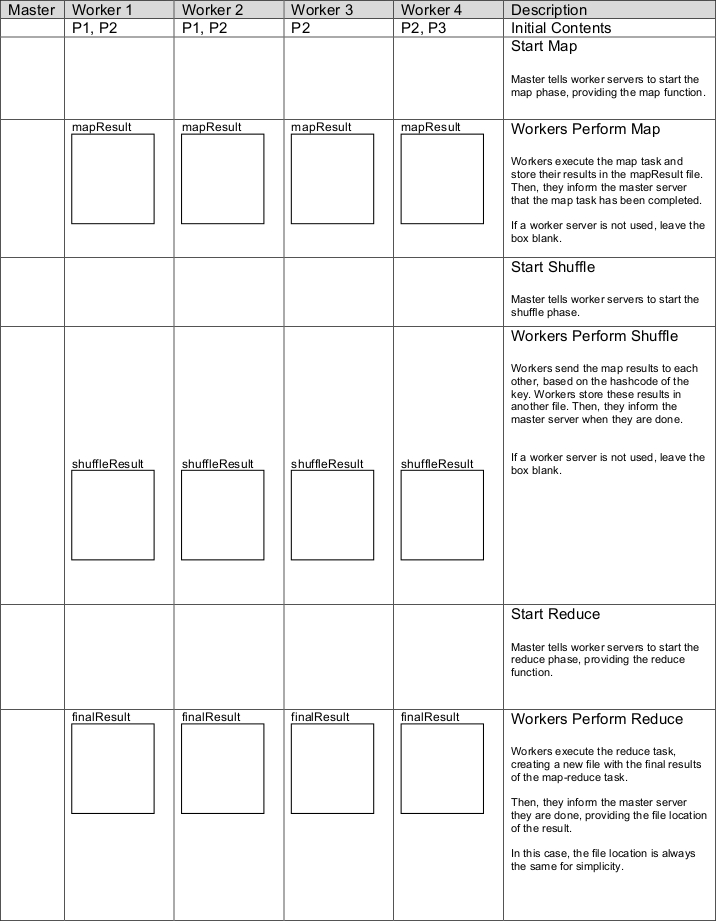
\includegraphics[width=6in]{map-reduce-diagram.jpg}

\end{document}
